\documentclass[11pt,letterpaper]{article}

\usepackage[utf8]{inputenc}
\usepackage[letterpaper,margin=2.35cm]{geometry}
\usepackage{amsmath}
\usepackage{booktabs}
\usepackage{tabularx}
\usepackage{xcolor}
\usepackage{graphicx}
\usepackage{hyperref}

\definecolor{azulprofundo}{HTML}{123047}
\definecolor{azullago}{HTML}{167D9A}
\definecolor{aguamarina}{HTML}{47B8A6}
\definecolor{gristexto}{HTML}{445D68}
\hypersetup{colorlinks=true,linkcolor=azullago,urlcolor=azullago,citecolor=azullago}
\setlength{\parindent}{0pt}
\setlength{\parskip}{0.65em}
\pagestyle{plain}
\renewcommand{\abstractname}{Resumen}
\renewcommand{\tablename}{Tabla}
\renewcommand{\figurename}{Figura}
\renewcommand{\refname}{Referencias}

\title{\vspace{-1.5cm}\color{azulprofundo}\textbf{Monitoreo satelital de cianobacterias\\en los lagos Atitlán y Amatitlán}\\[0.45em]
\large Informe de avance metodológico}
\author{Grupo 1}
\date{13 de agosto de 2026}

\begin{document}
\maketitle

\begin{abstract}
Este avance establece un procedimiento reproducible para observar cambios potenciales de cianobacterias en los lagos Atitlán y Amatitlán mediante imágenes Sentinel--2. Se definieron las áreas de estudio, se registraron las 22 fechas oficiales y se construyó un flujo que calcula tres indicadores sin descargar escenas satelitales completas. Los resultados numéricos y ambientales se incorporarán únicamente después de verificar las imágenes, las máscaras de nubes y la cobertura efectiva de cada lago.
\end{abstract}

\section{Pregunta ambiental}

Las floraciones de cianobacterias pueden afectar los ecosistemas, el abastecimiento de agua, la recreación y el turismo. La observación satelital permite revisar todo el espejo de agua de manera periódica, aunque sus estimaciones deben interpretarse como señales indirectas y no como sustitutos de un muestreo de campo.

El objetivo es describir cómo cambia la señal asociada con cianobacterias a través del tiempo y dentro de cada lago, así como explorar su relación con indicadores de vegetación y agua.

\section{Datos y cobertura temporal}

Se utilizará la colección Sentinel--2 L2A de Copernicus. La guía establece once fechas por lago entre enero de 2025 y julio de 2026. La selección de fechas se conserva exactamente en el archivo de configuración del proyecto para evitar diferencias entre integrantes.

\begin{table}[h]
\centering
\caption{Diseño del conjunto de observaciones.}
\begin{tabularx}{\textwidth}{lccX}
\toprule
\textbf{Lago} & \textbf{Fechas} & \textbf{Resolución} & \textbf{Observación de calidad} \\
\midrule
Atitlán & 11 & 20 m & Nubosidad oficial entre 0.01\% y 4.96\%. \\
Amatitlán & 11 & 20 m & La fecha 07-02-2026 tiene cerca de 57.1\% de cobertura válida. \\
\bottomrule
\end{tabularx}
\end{table}

Los GeoJSON entregados por el curso reproducen las cajas envolventes indicadas en la guía y se utilizan para limitar la consulta. Como son rectángulos y no siguen la orilla, para excluir el terreno circundante se incorporaron los contornos de las relaciones 5781818 y 11018382 de OpenStreetMap. Los primeros documentan la extensión oficial de búsqueda; los segundos permiten recortar el espejo de agua y calcular superficies.

\section{Procesamiento propuesto}

Para reducir almacenamiento y tiempo de transferencia, el procesamiento se ejecuta en CDSE mediante openEO. Se consultan únicamente las bandas azul (B02), verde (B03), roja (B04), infrarroja cercana (B08) y la clasificación de escena (SCL). Las salidas se remuestrean a 20 m y contienen tres productos derivados:

\begin{align}
\mathrm{NDVI} &= \frac{B08-B04}{B08+B04}, \\
\mathrm{NDWI} &= \frac{B03-B08}{B03+B08}, \\
\mathrm{CYA} &= 115530.31\left(\frac{B03\,B04}{B02}\right)^{2.38}.
\end{align}

NDVI ayuda a distinguir vegetación; NDWI resalta agua; CYA reproduce el modelo empírico del script Se2WaQ para Sentinel--2 L2A. Antes de calcular CYA, los valores enteros de Sentinel--2 se convierten a reflectancia con un factor de 0.0001.

\section{Control de calidad}

Se excluyen píxeles sin información, saturados, con sombra de nube, nubes de probabilidad media o alta, cirros y nieve según SCL. También se exigen reflectancias positivas en las cuatro bandas, evitando divisiones inestables e índices normalizados fuera del intervalo esperado. La máscara acuática inicial sigue el criterio de Se2WaQ y conserva NDWI mayor o igual que cero. Las ausencias se mantienen como datos faltantes y no se reemplazan con cero, pues hacerlo reduciría artificialmente los promedios.

Cada imagen será inspeccionada visualmente. También se calculará el número de píxeles válidos por fecha para reconocer cambios de cobertura. La observación parcial de Amatitlán del 7 de febrero de 2026 se reportará separadamente y no se comparará sin advertencia con imágenes completas.

\section{Resultados temporales preliminares}

Se descargaron y auditaron las 22 observaciones oficiales: once por lago, todas con tres bandas derivadas, proyección UTM 15N y resolución de 20 m. Los índices normalizados permanecieron en sus intervalos esperados. La cobertura válida estimada sobre el contorno del espejo de agua varió entre 77.7\% y 97.5\% en Amatitlán, y entre 43.2\% y 98.4\% en Atitlán. La imagen de Atitlán del 18 de enero de 2025 requiere especial cautela por su cobertura parcial.

La fórmula Se2WaQ puede producir valores extremos cuando la reflectancia azul es muy pequeña. Por ello, el ráster crudo se conserva para trazabilidad, pero las medias comparativas se calcularon sobre la escala publicada de 0 a 100. Esta decisión evita que pocos píxeles inestables oculten el patrón general y deberá someterse a un análisis de sensibilidad.

Como aproximación exploratoria, se probará un umbral de CYA igual a 40 unidades de $10^3$ células/ml, tomado de la escala gráfica de Se2WaQ. El porcentaje de agua por encima de ese valor ayudará a distinguir una señal intensa pero localizada de una señal extendida. Este umbral no se presentará como límite sanitario y se evaluará su sensibilidad.

\begin{figure}[h]
\centering
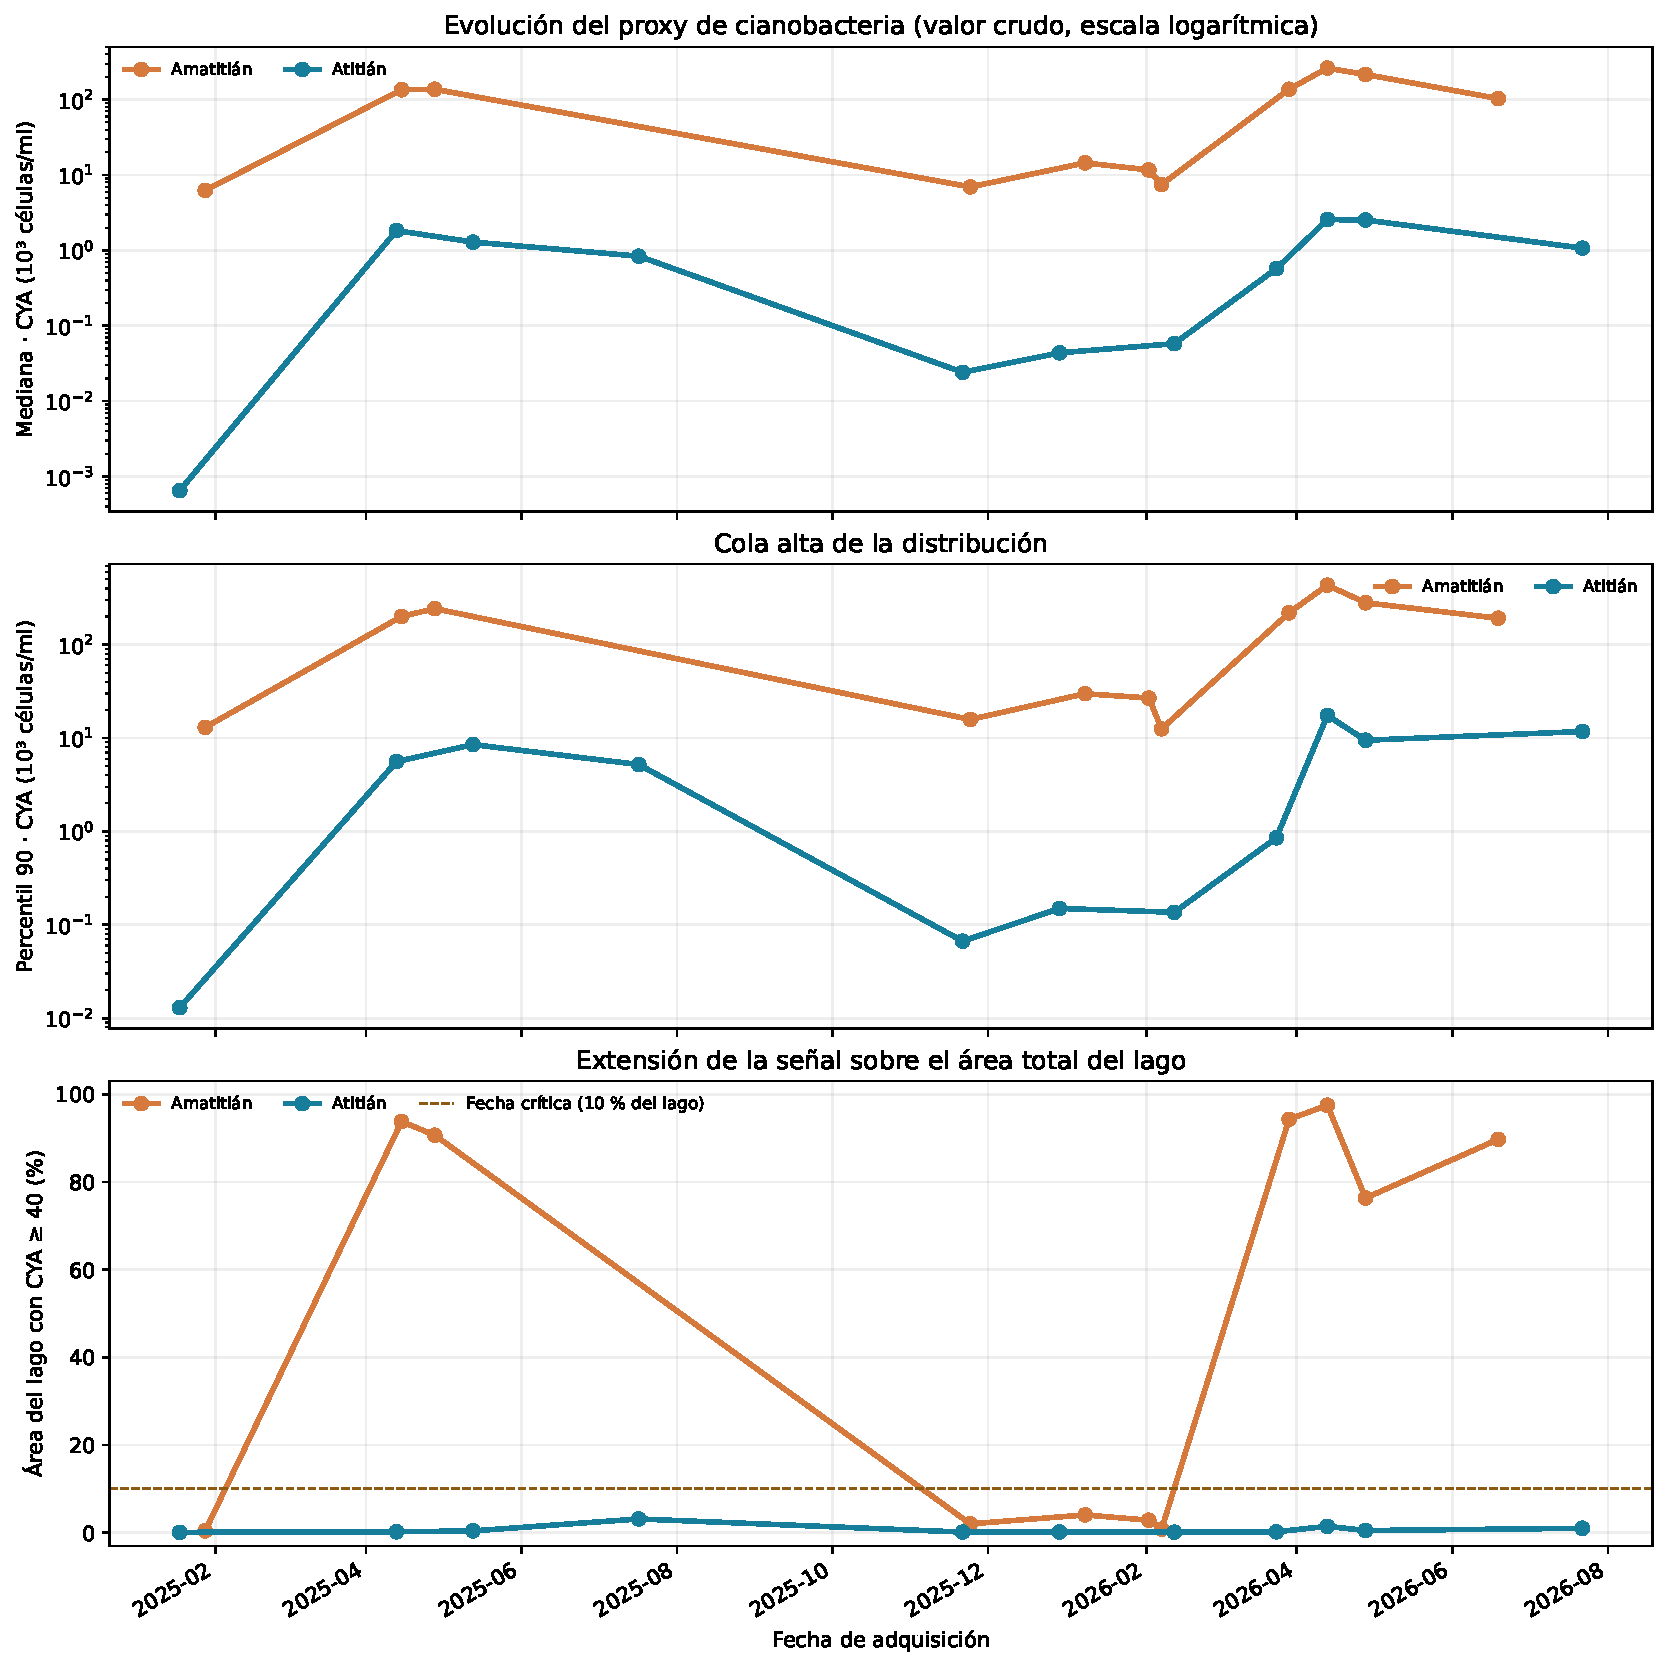
\includegraphics[width=\textwidth]{../outputs/figures/serie_temporal_cya.pdf}
\caption{Evolución temporal del proxy CYA medio y de la proporción válida con CYA mayor o igual a 40.}
\end{figure}

Amatitlán presenta señales altas y extendidas en abril de 2025 y nuevamente entre marzo y junio de 2026. Su máximo preliminar ocurre el 13 de abril de 2026, con media truncada de 99.1 y 99.97\% de la superficie válida por encima del umbral exploratorio. En Atitlán las señales son considerablemente menores y más localizadas; su máximo promedio provisional también ocurre el 13 de abril de 2026, con media 6.19 y 1.49\% por encima del umbral. Estos patrones no confirman por sí solos una floración ni una concentración real: describen la respuesta del modelo empírico aplicado a imágenes satelitales.

\section{Estado del avance y trabajo pendiente}

Se completaron la estructura versionable, las 22 descargas, el control de calidad inicial, las estadísticas temporales y mapas comparativos preliminares. Falta revisar manualmente todas las fechas, efectuar correlaciones, análisis de persistencia y comparación ambiental, y validar la robustez del modelo ante valores extremos.

\begin{thebibliography}{9}
\bibitem{potes2018}
Potes, M. y colaboradores (2018). \textit{Use of Sentinel 2--MSI for water quality monitoring at Alqueva reservoir}. Proceedings of the International Association of Hydrological Sciences, 380, 73--79.

\bibitem{se2waq}
Pereira, N. S. A. (2020). \textit{Se2WaQ -- Sentinel--2 Water Quality Script}. Sentinel Hub Custom Scripts. \url{https://custom-scripts.sentinel-hub.com/custom-scripts/sentinel-2/se2waq/}

\bibitem{cdse}
Copernicus Data Space Ecosystem. \textit{openEO API documentation}. \url{https://documentation.dataspace.copernicus.eu/APIs/openEO/openEO.html}

\bibitem{osm}
OpenStreetMap contributors. Contornos de los lagos Atitlán y Amatitlán, relaciones 5781818 y 11018382. Datos bajo licencia ODbL 1.0. \url{https://www.openstreetmap.org/copyright}
\end{thebibliography}

\end{document}
